\documentclass[12pt,letterpaper]{article}
\usepackage[spanish]{babel} % Para caracteres en español
\usepackage[utf8]{inputenc}	% Para caracteres en español
\spanishdecimal{.}
\usepackage[dvipsnames, table]{xcolor}
\usepackage{amsmath,amsthm,amsfonts,amssymb,amscd}
\usepackage{multirow,booktabs}
\usepackage{fullpage}
\usepackage{lastpage}
\usepackage[shortlabels]{enumitem}
\usepackage{fancyhdr}
\usepackage{bm}
\usepackage{mathrsfs}
\usepackage{wrapfig}
\usepackage{setspace}
\usepackage{calc}
\usepackage{multicol}
\usepackage{cancel}
\usepackage[retainorgcmds]{IEEEtrantools}
\usepackage[margin=2cm]{geometry}
\usepackage{graphics}
\usepackage{graphicx}
\usepackage{floatrow}
\usepackage{listings}
\usepackage{amsmath, xparse}
\newlength{\tabcont}
\setlength{\parindent}{0.0in}
\setlength{\parskip}{0.05in}


\title{}


% Editar como se necesite para cambiar los títulos
\newcommand\course{Optimization}
\newcommand\yourname{}% <-- nombre del curso

\theoremstyle{definition}
\newtheorem{defn}{Definición}
\newtheorem{reg}{Regla}
\newtheorem{ejer}{EJERCICIO}
\newtheorem{dem}{Proof}
\pagestyle{fancyplain}
\headheight 32pt
\rhead{\yourname}
\chead{\textbf{\Large Second Problem Set
}}
\lhead{Optimization UB 2022}
\textheight 610pt
\headsep 10pt
\footskip 40pt
\topmargin = 3pt

\begin{document}

\textbf{Exercise 1} 
Consider the problem 
$$\begin{aligned}
\min_{x\in \mathbb{R}^2} f(x) = -x_1  \quad \text{subject to} \quad 
& h_1(x) = (1-x_1)^3 -x_2 \geq 0 \\
& h_2(x) = x_1 \geq 0 \\
& h_3(x) = x_2 \geq 0 \\
\end{aligned}$$
Prove that $\mathcal{Z}^1(x^*) \cap \mathcal{Z}^2(x^*) \neq \emptyset$.

We can easily see that the point $x^* = (1, 0)^T$ is a local minimum under the imposed constraints. (We have also seen it in class.)
\\\\The set $\mathcal{I}(x):= \{j: h_j(x) = 0\}$, then we can easily check that $\mathcal{I}(x^*) = \{1, 3\}$.
\\Since the problem has no equality constraints, the linearizing cone at $x^*$ is defined as $$\mathcal{Z}^1(x^*) = \{z\,|\, z^T\nabla h_k(x^*)\geq 0 \,\text{ if } k\in \mathcal{I}(x^*)\}$$ and $$\nabla h_1(x) = (-3(1-x_1)^2\,, -1)^T \Longrightarrow \nabla h_1(x^*) = (0\,, -1)^T\,,$$ $$\nabla h_3(x) = (0\,, 1)^T \Longrightarrow \nabla h_3(x^*) = (0\,, 1)^T\,.$$ Then, for $z=(z_1\,, z_2)^T$ we obtain $$z^T\nabla h_1(x^*)\geq 0 \Longleftrightarrow \begin{bmatrix} z_1 & z_2 \end{bmatrix}\begin{bmatrix}0 \\ -1 \end{bmatrix} = -z_2 \geq 0\,,$$ $$z^T\nabla h_3(x^*)\geq 0 \Longleftrightarrow \begin{bmatrix} z_1 & z_2 \end{bmatrix}\begin{bmatrix}0 \\ 1 \end{bmatrix} = z_2 \geq 0\,,$$ meaning that $\mathcal{Z}^1(x^*) = \{z\,|\, z_2 = 0\}$.
\\\\Now, $\mathcal{Z}^2 = \{z \,|\,z^T\nabla f(x^*)<0\}$ and $\nabla f(x^*) = (-1\,, 0)^T$, then $$z^T\nabla f(x^*) < 0 \Longleftrightarrow \begin{bmatrix} z_1 & z_2 \end{bmatrix}\begin{bmatrix}-1 \\ 0 \end{bmatrix} = -z_1 < 0\,,$$ meaning that $\mathcal{Z}^2 = \{z \,|\,z_1>0\}\,.$
\\\\With these results, $\mathcal{Z}^1(x^*)\cap \mathcal{Z}^2(x^*) = \{z\,|\, z_1 >0\,, z_2=0\}\neq \emptyset\,.$
\\
\textbf{Exercise 2} 
\textbf{Exercise 2} \\
First, we write the generalized Lagrangian function associated to this problem: 
$$\mathcal{L}(x_1, x_2, \mu) = f(x_1, x_2) -\mu h(x_1,x_2) = (x_1-1)^2+x_2^2-\mu(- x_1 +\beta x_2^2)$$
According to Karush-Kuhn-Tucker theorem, $\exists x_1^*, x_2^*, \mu^*$ such that $\nabla\mathcal{L}(x_1^*, x_2^*, \mu^*)=0$
{\small
\begin{equation*}
    \begin{cases}
    \frac{\partial \mathcal{L}(x_1, x_2, \mu)}{\partial x_1} = 2x_1-2+\mu =  0 \\
     \frac{\partial \mathcal{L}(x_1, x_2, \mu)}{\partial x_2} = 2(1-\mu\beta)x_2 = 0 \\
     \frac{\partial \mathcal{L}(x_1, x_2, \mu)}{\partial \mu} = x_1-\beta x_2^2 = 0
    \end{cases}
\end{equation*}}\\
Take the second equation. This can only be satisfied either when $x_2=0$ or $(1-\mu\beta)=0$. 
\begin{itemize}
    \item For the solution when $x_2=0$, we get that $x_1=0$ by substitution in the third equation and $\mu=2$, by substituting $x_1=0$ in the first equation. We see that this solution is independent of the value that $\beta$ takes. The minimum achieved is $f^*(x_1, x_2) = 1$. 
    \item For the solution when $(1-\mu\beta)=0$ we get that $\mu = \frac{1}{\beta}$. By substituting $\mu$ in the first equation we get $x_1 = 1 -\frac{1}{2\beta}$ and by substituting $x_1$ in the third equation we get that $x_2 = \pm \sqrt{\frac{2\beta-1}{2\beta^2}}$. In order to have a solution in the reals, we need that $2\beta-1\geq0$. Hence, $\beta \geq \frac{1}{2}$. The minimum achieved is $f^*(x_1, x_2) = (1 -\frac{1}{2\beta} - 1)^2 + (\pm \sqrt{\frac{2\beta-1}{2\beta^2}})^2 = \frac{4\beta-1}{4\beta^2} $. 
\end{itemize}
I have plotted the objective function together with the constraint function for different values of $\beta$. The bigger the $\beta$, the greater the weight of the nonlinear term $x_2^2$ and the more pronounced the curvature of the constraint surface. The closer $\beta$ gets to zero, the more similarity to the plane $x_1 = 0$ we get.\\
Then, we compute the Hessian and we get:
$$ \mathcal{H}_{x_1x_2} (x_1, x_2, \mu) = 
\begin{bmatrix}
    2 & 0 \\
    0 & 2(1-\mu \beta) \\
\end{bmatrix}
$$
Now, we evaluate the candidate points and we see that $(x_1=0, x_2=0, \mu = 2)$ is a minimum for $\beta < \frac{1}{2}$ (this is the interval where the Hessian is positive definite) and that ($x_1 = 1 -\frac{1}{2\beta}$, $x_2 =  \pm \sqrt{\frac{2\beta-1}{2\beta^2}}$,  $\mu = \frac{1}{\beta}$) are both minima when $\beta  \geq \frac{1}{2}$ (the Hessian is positive definite and the solution is inside the reals).
\\

\textbf{Exercise 3} 

\textbf{If $(\hat{x}, \hat{\lambda}, \hat{\mu})$ is a solution of ($S$) then $\hat{x}$ is a solution of ($P$). Fullfil the details from the notes in class.}
\begin{equation}
     \sum_{j=1}^{m} (\hat{\lambda_j}-\lambda_j)g_j(\hat{x}) + \sum_{j=1}^{p} (\hat{\mu_j}-\mu_j)h_j(\hat{x}) \leq 0
\end{equation}

\begin{equation}
     f(\hat{x}) \leq f(x) + \sum_{j=1}^{m} \hat{\lambda_j}(g_j(\hat{x}) - g_j(x)) + \sum_{j=1}^{p} \hat{\mu_j}(h_j(\hat{x} - h_j(x))
\end{equation}
From definition, we also have that $\mu \geq 0 $.

And we would like to conclude that $g_j$ and $\hat{\mu}_j$ are the following in order to proof that $\hat{x}$ is a solution of $P$:
$$g_j(\hat{x})=0, j=1,...,m \ and \ \hat{\mu_j}h_j(\hat{x})=0, j=1,...,p $$.

So, we will prove it by contradiction. Using (1), we can state that $\mu_j = \hat{\mu}_j$ in order to eliminate from our equation the second part and play only with the first one. Therefore, we need to see if the following always holds:
$$\sum_{j=1}^{m} (\hat{\lambda_j}-\lambda_j)g_j(\hat{x}) \leq 0$$

If we first suppose that $g_j(\hat{x})>0$ and $\hat{\lambda}_j > \lambda_j$ we see how the left side of the inequation does not hold because it is positive. Similar, if we suppose that $g_j(\hat{x})<0$ and $\hat{\lambda}_j < \lambda_j$ does not hold too. Hence, $g_j(\hat{x}) = 0$ strictly in order to (1) be true.

Once here, we can go again to (a) and play now only with the second part:
$$\sum_{j=1}^{p} (\hat{\mu_j}-\mu_j)h_j(\hat{x}) \leq 0$$

First of all, suppose that $\mu_j = 0$ and then what needs to hold is $\sum_{j=1}^{p} \hat{\mu_j}h_j(\hat{x}) \leq 0$. By definition, $\mu \geq 0$, so must be $h_j \leq 0$. On the other hand, if now we suppose that $\hat{\mu_j} < \mu_j$, we need that $h_j \geq 0$. The following ends to:
$$\sum_{j=1}^{p} \hat{\mu_j}h_j(\hat{x})-\mu_j h_j(\hat{x}) \leq 0$$

Where we have said that the first part with $\hat{\mu}$ needs to be $\leq 0$, but if we use a $\mu_j$ bigger than $\hat{\mu}_j$ we arrive to a contradiction because $h_j$ cannot be negative and at the same time be positive, thus making $\hat{\mu_j}h_j(\hat{x}) = 0$. Then $\mu_j$ can be positive and $h_j$ can also be positive holding the inequation correctly.



\textbf{Exercise 4. Prove that the intersection of an arbitrary family of convex sets is also a convex set.} 

Let $\mathcal{C}_i$ be a convex set for $i \in \mathcal{I} $.
\\ 
Now let's define the intersection of $\mathcal{C}_i $ as $\bigcap_{i \in \mathcal{I}} \mathcal{C}_i$, we will prove that the intersection is a convex set as well.
\\
Let's take two points $u_1, u_2 \in \bigcap_{i \in \mathcal{I}} \mathcal{C}_i$, then the intersection is a convex set if 
$$
\alpha u_1 + (1- \alpha) u_2 \in \bigcap_{i \in \mathcal{I}} \mathcal{C}_i, \quad \alpha \in [0, 1], \quad \forall \ u_1, u_2 \in \bigcap_{i \in \mathcal{I}} \mathcal{C}_i.
$$
\\
We know that $u_1, u_2 \in \mathcal{C}_i \ \forall i$, since if they belong to the intersection of the sets they will also belong to the sets themselves, and since $\mathcal{C}_i \ \forall i$ is convex, 
$$
\alpha u_1 + (1- \alpha) u_2 \in \mathcal{C}_i \ \forall i, \quad \alpha \in [0, 1], \quad \forall \ u_1, u_2 \in \mathcal{C}_i
$$
and therefore
$$
\alpha u_1 + (1- \alpha) u_2 \in \bigcap_{i \in \mathcal{I}} \mathcal{C}_i, \quad \alpha \in [0, 1], \quad \forall \ u_1, u_2 \in \bigcap_{i \in \mathcal{I}} \mathcal{C}_i.
$$.


\textbf{Exercise 5. Denote by $\mathbb{C}$(G) the convex hull of an arbitrary set G $\subset$ $\mathbb{R}^n$.}

    
    Let $G \subset \mathbb{R}^n$ be an arbitrary set. The intersection of all convex sets containing G is called convex hull of G and it is denoted by $\mathcal{C}(G)$.
    
    Let's compute the convex hulls of the following sets:
\begin{itemize}
    \item $G= \{\cup_{n=1}^{3}(x_{n},y_n)\}\subset \mathbb{R}^2$
    %%%%%%%%%%
    
    C(G) is the area enclosed by the triangle formed by the three points in $\mathbb{R}^2$: $(x_1,y_1)$, $(x_2,y_2)$ and $(x_3,y_3)$. It is the smallest convex set containing G.
     \end{itemize}
    \begin{figure}[H]
        \centering
        \includegraphics[scale=0.06]{Imagen de WhatsApp 2022-11-21 a las 18.44.33.jpg}
        \caption{Convex hull of $G= \{\cup_{n=1}^{3}(x_{n},y_n)\}\subset \mathbb{R}^2$}
    \end{figure}
    
    \begin{itemize}
    
    \item Set $G_1=\{z=(x,y)\in \mathbb{R}^2\text{ }|\text{ }|z|<1\}$, $G_2$ to be the triangle whose vertices are the points A=(-2,0), B=(2,0) and C=(0,2), $G_3=\{z=(x,y)\in \mathbb{R}^2\text{ }|\text{ }x=-2 \text{ and }1\leq y \leq 2\}$. Consider $G=\cup_{n=1}^{3}G_n$.
    
    The convex hull of $G=\cup_{n=1}^{3}G_n$ will be the area enclosed by the points A=(-2,0), (-2,2), C=(0,2), B=(2,0) and the arch joining A and B passing by (0,-1) enclosing in this way $G_1$. It would correspond to the intersection of all convex sets containing G. Therefore, if two points belonging to the boundary of the convex hull are selected, all the points of the straight line that join those two points will belong to the convex hull.
        
    \end{itemize}
    \begin{figure}[H]
        \centering
        \includegraphics[scale=0.06]{Imagen de WhatsApp 2022-11-22 a las 09.29.44.jpg}
        \caption{Convex hull of $G=\cup_{n=1}^{3}G_n$}
    \end{figure}
    %%%%%%%%%%
      
\hfill\break

\textbf{Exercise 6} 

Suppose $f : D \subset \mathbb{R}^n \to \mathbb{R}$ be a $C^1$ function. Let $p^k$ be a
descent direction at the point $x_k \in D$ and assume $f |L_{p_k}$ is bounded
below where $L_{p_k} = \{x \in \mathbb{R}^n | x = x_k + \alpha p_k , \alpha > 0\}$. Then if
$0 < c_2 < c_1 < 1$ there may be no step
lengths that satisfies the Wolfe conditions.

Consider the convex function as on the graph and let us choose $c_1=0.99$. 
\begin{figure}[H]
    \centering\includegraphics[width=15cm,scale=0.8]{ {zdj} }
\end{figure}
\noindent Observe that the sufficient decrease line intersects the function only once.
In addition, for all points to the left of the intersection, we have: $\phi'(\alpha)\leq-\frac{1}{2}$.
Suppose that we choose $c_2=0.1$ so that the curvature condition requires: $\phi'(\alpha)\geq-0.1$.
Hence, in this case there is no step length $\alpha$ that satisfies the Wolfe conditions.

\textbf{Exercise 7} 
\textit{Solution}\\

\textbf{Exercise 8} 
In this case, we need to prove:
$$
(1-\lambda)f(x^*) + \lambda f(x) \geq f((1-\lambda)x^* + \lambda x)
$$
Now, lets put $f(x) = e^{ax}$ in the formula.
$$
(1-\lambda) e^{ax} + \lambda e^{ax} \geq e^{a((1- \lambda)x^*+\lambda x)}
$$
We assume $ax^* \geq ax$, so we can divide by $e^{ax}$.
\[
\begin{array}{c}
(1-\lambda) e^{ax^* - ax} + \lambda \geq e^{ax(1- \lambda)+ ax^* (1 - \lambda)} \\
(1-\lambda) e^{a(x^* - x)} + \lambda \geq e^{(1-\lambda)a(x^* - x)}
\end{array}
\]
Because $ax^* \geq ax$, we can now say: $s = a(x^* - x) > 0$, which gives us:
$$
(1-\lambda)e^s + \lambda \geq e^{(1-\lambda)s}
$$
Now we will compute Taylor Series of both sides, which gives us:
\[
\begin{array}{c}
(1-\lambda)e^s + \lambda = 1 + (1-\lambda)s + \frac{1}{2}(1-\lambda)s^2 + \frac{1}{6}(1-\lambda)s^3 + ... \\
e^{(1-\lambda)s} = 1 + (1-\lambda)s + \frac{1}{2}(1-\lambda)^2s^2 + \frac{1}{6} (1 - \lambda)^3 s^3 + ...
\end{array}
\]
We know $0 \leq \lambda \leq 1 \rightarrow 1 - \lambda \in [0,1]$ and $s>0$. So for $n \geq 0$ we have:
\[
\begin{array}{c}
(1-\lambda)s^n \geq (1-\lambda)^n s^n \\
1 + (1-\lambda)s + \frac{1}{2}(1-\lambda)s^2 + \frac{1}{6}(1-\lambda)s^3 + ... \geq  1 + (1-\lambda)s + \frac{1}{2}(1-\lambda)^2s^2 + \frac{1}{6} (1 - \lambda)^3 s^3 + ...
\end{array}
\]
And that is exactly what we want to proof.

\textbf{Exercise 9} 
\textit{Solution}\\

\textbf{Exercise 10. Let $f$ be a convex function. Prove that the set of global minimizers of $f$ forms a convex set.
} 

Let's consider the set $\mathcal{S} = \{x^* : f(x^*) = \delta \} $, representing the set of global minimizers of $f$, where $\delta$ is the value of $f$ at the minimizing points. Let's take any $u_1, u_2 \in \mathcal{S}$, then for the convexity of $f$ and for $\alpha \in [0,1]$
$$f(\alpha u_1 + (1- \alpha) u_2 )\leq \alpha f(u_1) +(1- \alpha) f(u_2)$$.
\\
Furthermore we can say that 
$$  \alpha f(u_1) +(1- \alpha) f(u_2) = \alpha \delta +(1-\alpha) \delta = \delta.$$
\\
Therefore we can say that  $ f(\alpha u_1 + (1- \alpha) u_2 )\leq \delta$ and that  $$ \alpha u_1 + (1- \alpha) u_2 \in \mathcal{S}, \quad \forall u_1, u_2 \in \mathcal{S}, \quad \alpha \in [0,1]. $$

%%%%%%%%%%%%%%%%%%%%
\textbf{Exercise 11. Consider the function $f(x_1, x_2) = (x_1 + x_2^2)^2$. At the point $\textbf{x}^T_0 = (1, 0)$ we consider the direction $\textbf{p}^T = (-1, 1)$. Show that $p^T$ is a descent direction and find all minimizers of the problem}
$$\min_{\alpha\in\mathbb{R}^+} f(\textbf{x}+\alpha\textbf{p})$$
%%%%%%%%%%%%%%%%%%%%%
Firstly, I will show that $\textbf{p}^T$ is a descent direction. We say that $p_k^T$ is a descent direction if $p_k\nabla f(\textbf{x}_k)<0$. 
$$\nabla f=(\frac{\delta f}{\delta x_1}, \frac{\delta f}{\delta x_2})=(2(x_1+x_2^2), 4x_2(x_1+x_2^2)) \longrightarrow \nabla f(x_0)=(2,0)$$
$$(-1, 1)^T\nabla f=(-1,1)^T(2,0)=-2<0$$
Therefore, $\textbf{p}^T$ is a descent direction.

Secondly, I will find the minimizers of $\min_{\alpha\in\mathbb{R}^+} f(\textbf{x}+\alpha\textbf{p})$:

In order to have a minimizer, we should have: $f'(\textbf{x}+\alpha\textbf{p})=0$ or $\nabla f(\textbf{x}+\alpha\textbf{p})^T\textbf{p}=0$ with $\textbf{x}^T_0 = (1, 0)$ and $\textbf{p}^T = (-1, 1)$:

$$\nabla f(\textbf{x}+\alpha\textbf{p})^T\textbf{p}=\nabla f(1-\alpha,\alpha)^T\textbf{p}=$$ $$=(2(1-\alpha+\alpha^2),4\alpha(1-\alpha+\alpha^2))·(-1,1)^T=(4\alpha-2)(1-\alpha+\alpha^2)=0 \longrightarrow \alpha=\frac{1}{2}$$

Therefore, the only minimizer is for $\alpha=\frac{1}{2}$ as it should be a real positive number.

\hfill\break

\textbf{Exercise 12} 
\begin{itemize}
    \item[a)]
    Assuming $p'(\alpha)\neq 0$ for $\alpha \in \mathbb{R}$
    \[N_p(\alpha)=\alpha-\frac{p(\alpha)}{p'(\alpha)}=\alpha \iff -\frac{p(\alpha)}{p'(\alpha)}=0 \iff p(\alpha)=0 \]
    \item[b)] Observe that $N'(x)=1-\frac{p'(x)^2-p(x)p''(x)}{p'(x)^2}=\frac{p(x)p''(x)}{p'(x)^2}$. If $\alpha$ is a simple root of $p(x)$ (assume that $\alpha=\alpha_w$ for $0\leq w \leq k$) then $p'(\alpha)\neq 0$ because
     \begin{equation}
     \begin{aligned}
        p'(x)&=q'(x)\prod_{j=1}^k (x-\alpha_j)^{m_j}+q(x)m_1(x-\alpha_1)^{m_1-1}\prod_{j=2}^k (x-\alpha_j)^{m_j}+...+ \\
        & +q(x)\prod_{j=1}^{w-1} (x-\alpha_j)^{m_j} \prod_{j=w+1}^k (x-\alpha_j)^{m_j} +...+q(x)m_k(x-\alpha_k)^{m_k-1}\prod_{j=1}^k-1 (x-\alpha_j)^{m_j}
     \end{aligned}
     \end{equation}
    \[p'(\alpha)=q(x)\prod_{j=1}^{w-1} (x-\alpha_j)^{m_j} \prod_{j=w+1}^k (x-\alpha_j)^{m_j}\neq 0\]
    Then $N'(p)=\frac{p(\alpha)p''(\alpha)}{p'(\alpha)^2}=0$ because $p(\alpha)=0$ and $p'(\alpha)\neq 0$. \\
    Let $\alpha$ be any simple root of $p$. Because polynomials and its derivatives are continuous functions $N'(p)$ is also continuous. That means there exists small enough $\delta>0$ such that $|x-\alpha|<\delta$ $\Rightarrow$ $|N'(x)|<\epsilon$ for all $\epsilon>0$ because we know that $N'(\alpha)=0$. From the Fixed point Theorem we have that for all $x_0\in(\alpha-\delta,\alpha+\delta)$ $x_n=N(p(x_{n-1}))\to x^*$, so the Newton method is always convergent in a sufficiently small neighbourhood of $\alpha$.
    \item[c)]
    Put $x_n=\alpha + \epsilon_n$, $x_{n+1}=\alpha + \epsilon_{n+1}$ (approximation of the root). Then the Newton method
    \begin{equation}
    \begin{aligned}
    x_{n+1}&=x_n-\frac{p(x_n)}{p'(x_n)} \iff \epsilon_{n+1}=\epsilon_n - \frac{p(\alpha+\epsilon_n)}{p'(\alpha+\epsilon_n)}=\epsilon_n - \frac{p(\alpha)+\epsilon_n p'(\alpha)+\frac{\epsilon_n^2 p''(\alpha)}{2!}}{p'(\alpha)+\epsilon_n p''(\alpha)}=\\ 
    &=\frac{\epsilon_n (p'(\alpha)+\epsilon_n p''(\alpha))-p(\alpha)-\epsilon_n p'(\alpha)-\frac{\epsilon_n^2 p''(\alpha)}{2!}}{p'(\alpha)+\epsilon_n p''(\alpha)}=\frac{\epsilon_n^2p''(\alpha)}{2p'(\alpha)(1+\frac{\epsilon_n p''(\alpha)}{p'(\alpha)})}= \\
    & (\frac{\epsilon_n p''(\alpha)}{p'(\alpha)} \quad \text{is very small})= \frac{\epsilon_n^2p''(\alpha)}{2p'(\alpha)}=\epsilon_n^2K \quad \text{where} \quad K=\frac{p''(\alpha)}{2p'(\alpha)}
    \end{aligned} 
    \end{equation}
    We obtain $\frac{|\epsilon_{n+1}|}{|\epsilon_n^2|}\to|K|>0$ when $n\to\infty$, so the convergence is quadratic.
\end{itemize}

\textbf{Exercise 13} 
$$p(x) = -18.8496 - 143.588x + 128.148x^2 + 113.355x^3 - 144.125x^4 + 24.7208x^5 + 19.634x^6 - 8.68x^7 + x^8 $$

\textbf{We know it has all roots belonging to $\Re$. Find intervals $[aj, bj ], j = 1,...,8$ in which there is one and only one root. Program a Newton mehtod to compute all roots with an error less than $10^-^6$}

As we can see, our algorithm has found correctly with a very high precision 6 of the 8 roots of this polynomial. It seems incapable to find the other two, which is strange using the Newton method and using multiple iteration with a wide range and diverse trials. Plotting the function we can easily see that there are only 6 real roots and the other 2 correspond to complex roots, more exactly and solved with an online calculator, are: $x_1 = 2.07225 - 0.0584619i$ & $x_2 = 2.07225 + 0.0584619i$. 

The code and results can be seen here (\ref{fig:code}). And at the image below (\ref{fig:plot}) we can see the function plotted.

\begin{figure}[H]
    \centering
    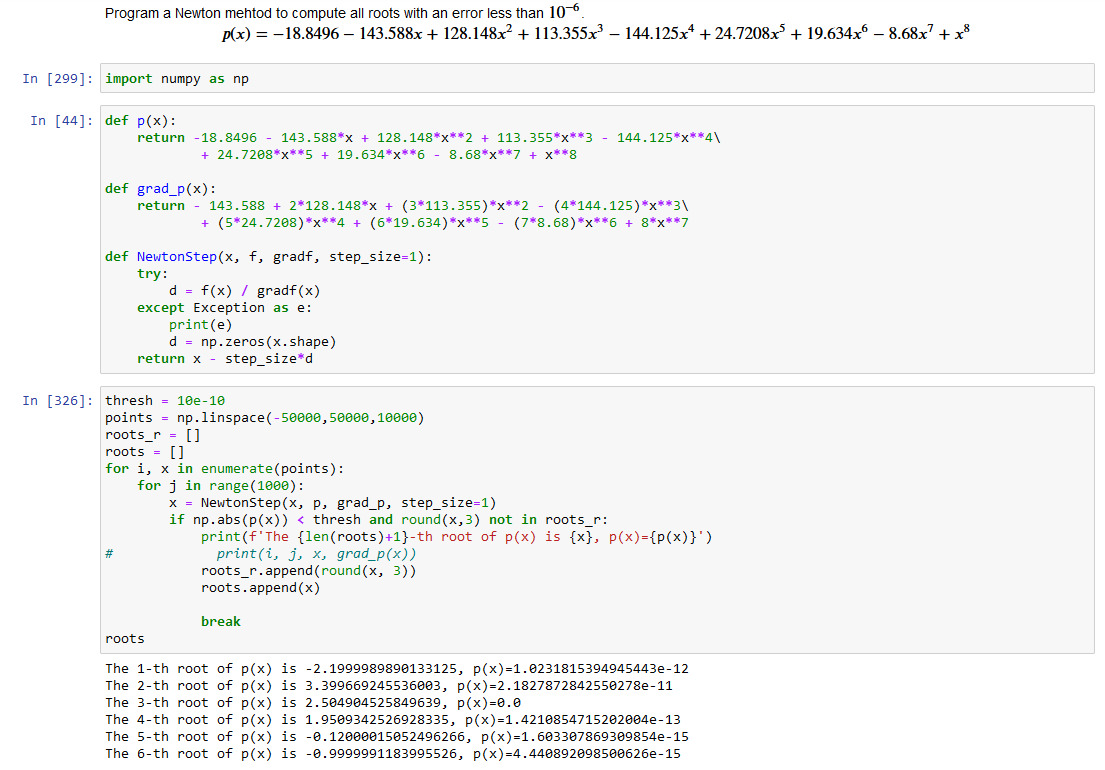
\includegraphics[width=1.1\textwidth]{code.jpeg}
    \decoRule
    \caption{Code and results for $p(x)$}
    \label{fig:code}
\end{figure}


\begin{figure}[H]
    \centering
    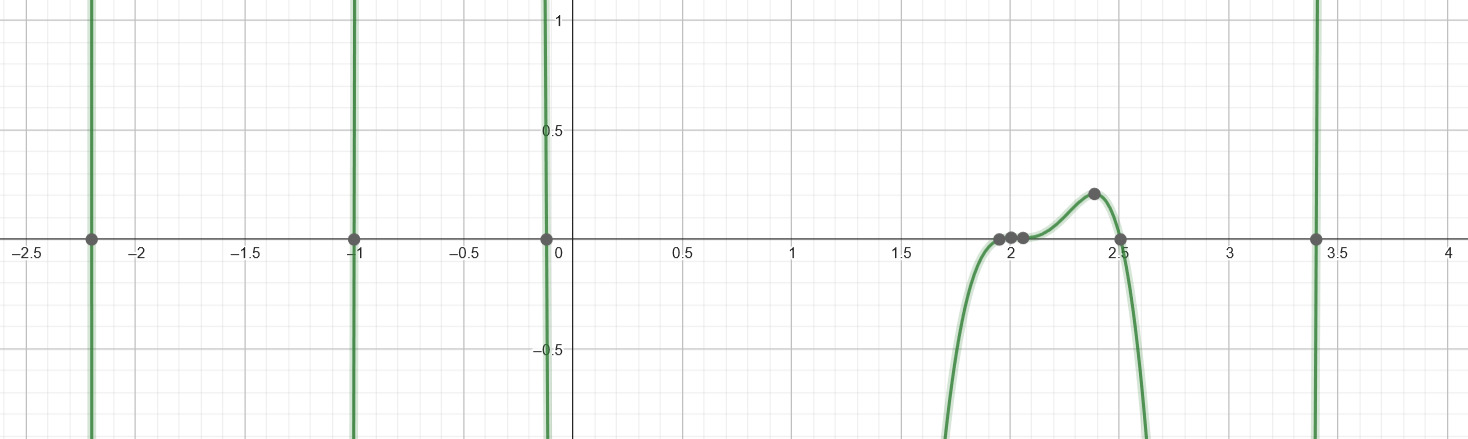
\includegraphics[width=1\textwidth]{plot.jpeg}
    \decoRule
    \caption{Function plot with an online calculator}
    \label{fig:plot}
\end{figure}

\\
\textit{An alternative solution}\\
To start with, I checked the roots of this polynomial with Wolfram Alpha, and discovered that there are only 6 real roots. Therefore, I will do this exercise taking into consideration this assumption. In the table below I have included the intervals with its corresponding root found with the Newton method. We see that the sign of the polynomial evaluated at the margins changes. We know that in each interval there is a root (Bolzano) and that it is unique because we only have 6 real roots.
\begin{table}[!h]
\begin{center}
\begin{tabular}{ |c|c|c|c| }
\hline
$[a_j, b_j ]$ & [$f(a_j) $,$f(b_j)$] & root\\
\hline
$[-2.7000, -1.7000]$ & [7375.7787, -616.2124] & -2.1999\\
$[-1.5000, -0.5000]$ & [-417.4848, 61.4101] & -0.9999 \\
$[-0.6200, 0.3800]$ & [70.3010, -51.4482] & -0.1200 \\
$[1.4509, 2.4509]$ & [-5.6220, 0.1551] & 1.9509 \\
$[2.0049, 3.0049]$ & [0.0080, -11.8339] & 2.5049 \\
$[2.8997, 3.8997]$ & [-7.7375, 545.7704] & 3.3996 \\
\hline
\end{tabular}
\end{center}
\end{table}\\
I include below the code that I used to compute the roots using the Newton method. This function takes as parameter a starting point. I decided to give for each interval as initial guess a uniform random number in the interval. As this algorithm is not bounded to a range, we always converge but not necessarily to the root inside the interval. By repeating the experiment several times, we eventually get a good starting point that leads to the root inside the interval.
\begin{lstlisting}[language=Python]
def newton_root_finding(x0, f, df, max_its=1000, tol=10e-6):
    x = x0
    fun = f(x)
    der = df(x)
    
    for i in range(max_its):
        x = x - (fun/der)
        if abs(fun)<=10e-6:
            break
        fun = f(x)
        der = df(x) 
    return x, i+1
\end{lstlisting}

\newcommand{\Lim}[1]{\raisebox{0.5ex}{\scalebox{0.8}{$\displaystyle \lim_{#1}\;$}}}
\textbf{Exercise 14} 
\subsection*{a}
The sequence of $x_k = \frac{1}{k!}$ converges superlinearly to $x^*$ if
$\Lim{k \to \infty} \frac{|x_{k+1}-x^*|}{|x_k - x^*|} = p$, where $p=0$. \newline
We can compute $\Lim{k \to \infty} x_k \rightarrow \Lim{k \to \infty} \frac{1}{k!} = 0$. This shows the sequence converges to 0. \newline
From here, we can fill in the values for $x^*$, which gives us:
$$
\Lim{k \to \infty} \frac{|x_{k+1}-0|}{|x_k-0|} = \Lim{k \to \infty} \frac{|x_{k+1}|}{|x_k|}  
$$
Now, let us plug in the value for $x_k$, and we get:
$$
\Lim{k \to \infty} \frac{\frac{1}{(k!+1)}}{\frac{1}{k!}} = \Lim{k \to \infty} \frac{k!}{(k+1)!} = \Lim{k \to \infty} \frac{k!}{(k+1)k!} = \Lim{k \to \infty} \frac{1}{k+1} = \frac{1}{\infty} = 0
$$
As we can see, p is in 0 in this case. This means we can say that $x_k = \frac{1}{k!}$ converges superlinearly to $x^* = 0$

\subsection*{b}
The sequence $x_k = 1+ (\frac{1}{2})^{2^k}$ converges quadratically if there is a positive constant C such that:
$$
\Lim{k \to \infty} \frac{|x_{k+1} - x^*|}{|x_k - x^*|^2} = C
$$
We can compute $\Lim{k \to \infty} x_k = \Lim{k \to \infty} 1 + (\frac{1}{2})^{2^k} = 1$. This shows the sequence converges to 1. Now, let us plug this value in. This gives us:
$$
\Lim{k \to \infty}  \frac{|x_{k+1} - 1|}{|x_k - 1|^2} = \Lim{k \to \infty}  \frac{|1 + (\frac{1}{2})^{2^{k+1}}- 1|}{|1 +(\frac{1}{2})^{2^k} - 1|^2} =  \Lim{k \to \infty} \frac{|(\frac{1}{2})^{2^{k+1}}|}{|(\frac{1}{2})^{2^k}|^2} = \Lim{k \to \infty} \frac{|\frac{1}{2^{k+1}}|}{|\frac{1}{2^{k*2}}|^2} = \Lim{k \to \infty} \frac{|2^{2^{k+1}}|}{|2^{2^{k+1}}|} = 1
$$
C is 1, which is bigger than 0 and therefore proves that the sequence converges quadratically to 1.\\

\textbf{Exercise 15 -  Let $f(x) = x^2+exp(x)-3.$} 

\quad a) Prove that f(x) = 0 has two and only two solutions.
\\
We know that for $f(x) = x^2 + e^x -3, \ f''(x) = 2+e^x$  assumes only positive values and therefore $f'(x) = 2x+e^x $ will be strictly increasing. 
\\
We can calculate easily $f'(-1) = \frac{1}{e} -2 < 0$ and $f'(0) = 1 > 0$, we also know that $f'(x)$ is continuous since the sum of two continuous functions is also continuous, and for Bolzano's theorem, since $f' : [-1, 0] \rightarrow \mathbb{R}$ is continuous and it satisfies $f'(-1)f'(0) < 0$, there will exist $c \in (-1, 0)$ such that $f'(c) = 0$.
\\
Since $f'(x)$ is strictly increasing and $f'(c) = 0, \ f(x)$ will have a minimum at $x = c.$ Then we can calculate 
$$
f(-2) = 1 + \frac{1}{e^2}  > 0, \quad
f(0) = -2 < 0, \quad
f(1) = e - 2 > 0.$$
By considering $f'(x)$, we can guess the behaviour of $f(x)$, that will decrease for $x \in (- \infty, c)$ and increase for $x \in (c, + \infty), \ c \in (-1, 0).$ Now there are three possible outcomes for $f(x)$: it can be strictly positive (never satisfying $f(x) = x^2 + e^x -3 =0$), non-negative (satisfying  $f(x) = x^2 + e^x -3 =0$ at $x=c$) or it assumes negative values  (satisfying  $f(x) = x^2 + e^x -3 =0$ in two points). Since we know that $f(0) = -2 < 0$ we can conclude that $f(x)$ has 2 and only 2 zeros at $x_0 \in (-2, c), \ x_1 \in (0, 1).$
\\ \\
\quad b) Find  appropriate fixed point methods (different from Newton method) to solve the equation
(show that the methods you have found satisfy the assumptions of the fixed point theorem (see
notes in class).
\\
Let's find the zeros of $f(x) = x^2+ e^x -3 = 0$ as fixed points of 
\\ $g_1(x) = \frac{3-e^x}{x} = x$ and $g_2(x)= ln (3-x^2)= x$.
\\ \\
- $g_1 : [-2, -1.8] \rightarrow [-2, -1.8] $ is continuous and differentiable, and it satisfies $|g_1'(x)| \leq k = 0.78 < 1 \ \forall x \in (-2, -1.8)$ since $|\frac{(1-x)e^x-3}{x^2}|< 1 \ \forall x \in (-2, -1.8)$. 

Then, for all $x_0 \in (-2, -1.8)$ we have $x_n := g_1(x_{n-1}) \rightarrow x^*$, with $g_1(x^*)=x^*.$
\\ \\
- $g_2 : [0, 0.9] \rightarrow [0, 0.9] $ is continuous and differentiable, and it satisfies \\ $|g_2'(x)| \leq k = 0.82 < 1 \ \forall x \in (0, 0.9)$ since $|\frac{2x}{x^2-3}|< 1 \ \forall x \in (0, 0.9)$. 

Then, for all $x_0 \in (0, 0.9)$ we have $x_n := g_2(x_{n-1}) \rightarrow x^*$, with $g_2(x^*)=x^*$.
\\ \\
\quad c)  Predict the number of iterates you should use to get the solutions (for each case) with an error
less than $10^{-6}$.
\\
For $g_1(x)$ the starting point will be $x=-1.9$ while for $g_2(x)$ it will be $x=0.5$

- $\frac{k^n}{1-k} |x_n - x_{n-1}| < 10^{-6}, \quad \frac{0.78^n}{0.22}|-1.50023-(-1.9)| < 10^{-6}, \quad n > 58$

- $\frac{k^n}{1-k} |x_n - x_{n-1}| < 10^{-6}, \quad \frac{0.82^n}{0.18}|1.0116-0.5| < 10^{-6}, \quad n > 74.88 \approx 75$
\\ \\
\quad d)  Do a program to compute the solutions and discuss the previous item.
\\
By looking at the solutions provided by the program that I wrote, the first function $g_1(x)$ takes 40 iterations while the second function $g_2(x)$ needs 36 iterations, in both cases the iterations needed are less than the estimated ones, and this is because of the bounds of the derivative.

%%%%%%%%%%%%%%%%%%%
\textbf{Exercise 16. Let $f(x)=x^2+exp(x)-3$.}
\begin{itemize}
    \item Prove that f(x)=0 has two (and only two) solutions.
    %%%%%%%%%%%
    
    Bolzano's Theorems says: Let $f : [a, b] \longrightarrow \mathbb{R}$ be a continuous function satisfying $f(a)f(b)< 0$. Then, there exists $x^* \in (a, b)$ such that $f(x^*) = 0$.
    
    The function is continuous in all the domain as is a sum of continuous functions ($x^2$, $e^x$, 3). Moreover,
    $$f(-2)=1.135\text{;    }f(-1)=-1.632\text{;      }f(0)=-2.0\text{;      }f(2)=8.389$$
    As $f(-2)f(-1)< 0$ and $f(0)f(2)< 0$, from Bolzano's Theorem, we can confirm that there exists at least one $x_1^* \in (-2, -1)$ and at least one $x_2^* \in (0, 2)$ such that $f(x_1^*)=f(x_2^*) = 0$.
    
    To show that they are unique and that, thus, $f(x)=0$ has only two solutions, I will use the following corollary: 
    
    Let $f : [a, b] \longrightarrow \mathbb{R}$ be a continuous function in [a, b] and derivable in (a, b). Assume that $f(a)f(b)< 0$ and $f'(x)\neq 0$ for all $x \in (a, b)$. Then, there exists a unique $x^* \in (a, b)$ such that $f(x^*) = 0$.
    
    The first derivative of f(x):
    $$f'(x)=2x+e^x$$ 
    The unique solution of $f'(x)=0$ is $x=-0.3517$. This point does not belong to any of the two intervals I considered. From the corollary, I can affirm that there are two and only two solutions of $f(x)=0$:
    $$x_1^* \in (-2, -1)\text{;   }x_2^* \in (0, 2)$$
    
    \item Find intervals $[a_j, b_j]$, j = 1, 2 where there is just one zero of f.
    
    I already proved in the previous task that there is just one solution of $f(x)=0$ in the following intervals:
    $$x_1^* \in (-2, -1)\text{;   }x_2^* \in (0, 2)$$
    
    \item Use Newton method to compute the solutions above and show that the sequence of iterates converges quadratically.
    %%%%%%%%%%%%%
\end{itemize}

Coding the Newton method with Python I got the following values for the different update steps. Getting as a final result: $x_n=-1.677233$. Moreover, it shows with the last column values of $|x_n-x_{n-1}|$ how the convergence is quadratic.
    \begin{table}[H]
    \centering
\begin{tabular}{c|c|c|c}
$x_n$ & $f(x_n$ & $f'(x_n)$ & $|x_n-x_{n-1}|$ \\
\hline
-2.0                      & 1.135335                    & -3.864665 & 2.0             \\
-1.706227                 & 0.092759                    & -3.230904 & 0.293773        \\
-1.677517                 & 0.0008998                   & -3.168196 & 2.8710e-2       \\
-1.677233                 & 8.819881                    & -3.167575 & 2.8401e-4       \\
-1.677233                 & 8.881784                    & -3.167575 & 2.7844e-8      
\end{tabular}
\end{table}


\section*{Problem 4} 

Given $C_i$ with $i \in I$ an arbitrary family of convex sets. We want to see that the intersection is also convex. A set $C$ is convex if for any two points in the set $u_1, u_2$, we have $\alpha u_1 + (1-\alpha) u_2 $ is in $C$ $\forall \alpha \in [0,1]$. 

Let's see that given $ u_1, u_2 \in \bigcap_{i\in I} C_i$ we have $\alpha u_1 + (1-\alpha) u_2 $ in $\bigcap_{i\in I} C_i$ $\forall \alpha \in [0,1]$. 

If $ u_1, u_2 \in \bigcap_{i\in I} C_i$ in particular they belong to all the sets $C_i$. As all $C_i$ are convex, then we have that $\alpha u_1 + (1-\alpha) u_2 $ is in $C_i$ $\forall \alpha \in [0,1]$. As this hold $\forall i \in I$ then we can afirm $\alpha u_1 + (1-\alpha) u_2 $ is in $\bigcap_{i\in I} C_i$ $\forall \alpha \in [0,1]$ just like we wanted to see. 

\section*{Problem 9}
 $\phi: \mathbb{R} \to \mathbb{R}$, defined as $\phi(\theta) = f(x_0+ \theta z)$. We consider $\phi \approx \hat{\phi}$. Where $\hat{\phi}(\theta) = a + b\theta + c \theta ^2 $.
 

 We know that $\hat{\phi}'(\theta) = b + 2c \theta $ and $\hat{\phi}''(\theta) = 2c $. $\theta^{*}$ to be the minimum has to verify: $\hat{\phi}'(\theta^{*}) = 0$ and $\hat{\phi}''(\theta^{*}) \ge 0$, which is equivalent to $\theta^{*} = - \frac{b}{2c}$ and $c\ge 0$. We are approximating the function with a quadratic form that is convex and has an unique minimum. The values of $a$,$b$,$c$ that describe the quadratic form can be obtained if we know 3 points of the function. If $\theta_1, \theta_2, \theta_3$ are the tree points where $f$ is evaluated then $a$, $b$ and $c$ are the solution of the following system:

 $$
\begin{pmatrix}
    1 & \theta_1 & \theta_1 ^2 \\
    1 & \theta_2 & \theta_2 ^2 \\
    1 & \theta_3 & \theta_3 ^2 \\
\end{pmatrix}
\begin{pmatrix}
    a \\
    b \\
    c\\
\end{pmatrix}
=
\begin{pmatrix}
    \hat{\phi}(\theta_1) \\
    \hat{\phi}(\theta_2) \\
    \hat{\phi}(\theta_3)\\
\end{pmatrix}
 $$
We don't need to arrive to the solution of $a$, as it is not used in the minimum. To solve the system we subtract row 2 and row 1, and we subtract row 3 and row 1. We multiply $ \theta_3-\theta_1$ to the resulting row 2 and $ \theta_2-\theta_1$ to the resulting row 3. Finally, subtracting row 3 and row 2 we arrive to the following system, from where $c$ can be isolated giving the inequality searched:

 $$
\begin{pmatrix}
    1 & \theta_1 & \theta_1 ^2 \\
    0 & (\theta_3 - \theta_1) (\theta_2 - \theta_1)  & (\theta_3 - \theta_1) (\theta_2 ^2-\theta_1^2) \\
    0 & 0 & (\theta_3 - \theta_1) (\theta_2 - \theta_1) (\theta_3 - \theta_2) \\
\end{pmatrix}
\begin{pmatrix}
    a \\
    b \\
    c\\
\end{pmatrix}
=
$$
$$
\begin{pmatrix}
    \hat{\phi}(\theta_1) \\
    (\theta_3 - \theta_1)\hat{\phi}(\theta_2) - (\theta_3 - \theta_1)\hat{\phi}(\theta_1)  \\
    (\theta_2 - \theta_1)\hat{\phi}(\theta_3) - \theta_2 \hat{\phi}(\theta_1)-\theta_3 \hat{\phi}(\theta_2) + \theta_1 \hat{\phi}(\theta_2) + \theta_3 \hat{\phi}(\theta_1) \\
\end{pmatrix}
 $$
 
$$
-c= \frac{(\theta_2-\theta_3)\hat{\phi}(\theta_1) + (\theta_3-\theta_1)\hat{\phi}(\theta_2)+ (\theta_1-\theta_2)\hat{\phi}(\theta_3)}{(\theta_3-\theta_1)(\theta_2-\theta_1) (\theta_3-\theta_2)} <0
$$

Substituting into the second equation we obtain:

$$
b =  \frac{(\theta_2^2-\theta_3^2)\hat{\phi}(\theta_1) + (\theta_3^2-\theta_1^2)\hat{\phi}(\theta_2)+ (\theta_1^2-\theta_2^2)\hat{\phi}(\theta_3)}{(\theta_3-\theta_1)(\theta_2-\theta_1) (\theta_3-\theta_2)}
$$

$$
\theta^{*} = - \frac{b}{2c} = \frac{(\theta_2^2-\theta_3^2)\hat{\phi}(\theta_1) + (\theta_3^2-\theta_1^2)\hat{\phi}(\theta_2)+ (\theta_1^2-\theta_2^2)\hat{\phi}(\theta_3)}{2[(\theta_2-\theta_3)\hat{\phi}(\theta_1) + (\theta_3-\theta_1)\hat{\phi}(\theta_2) + (\theta_1-\theta_2)\hat{\phi}(\theta_3)]}
$$
\section*{Problem 15}
Let $f(x) = x^2 + e^x -3 $
\vspace{0.5cm}
    To see that $f(x)=0$ has two (and only two) solutions, we will see that there is one solution in the interval $ ( -2, 0]$ and another in the $(0,0.9)$ and no more.

    As $f(-2) = 1.1353 >0 , f(0) =-2 <0, f(0.9) = 0.2696>0 $ applying  Bolzano's theorem we can say, there $\exists$  $c_1, \in ( -2, 0]$ and $c_2 \in (0, 0.9)$ such that $f(c_1) = f(c_2)=0$. Applying Rolle theorem, we can assure $\psi_1$ such that $f'(\psi_1) = 0$. $f'(x) = 2x + e^x $ and $f''(x) = 2 + e^x >0$. As $f''(x)$ is posivite, then $f'(x)$ is a monotonically increassing function. With that we can assure the $f'(x) = 0$ only at one point , $\psi_1$, otherwise there would be a change in the monotony and it's not the case. So if there exists another point $c_3$ such that $f(c_3)=0$, then using Rolle's theorem there exists another $\psi_2$ such that $f'(\psi_2)=0$, but we have already seen that this can not happens and $f$ has 2 and only 2 solutions.  

\vspace{0.5cm}

    Now that we know that is a solution of f, $c_1$, in the inteval $( -2, 0]$ and another one, $c_2$, in the inteval $(0, 0.9)$ we have to find one fixed point method to find each of them. 

    To find $c_1$, we will use the fixed point $g_1(x) =- \sqrt{3- e^x}$. 
    $g_1(x)=x \leftrightarrow x^2 = 3- e^x \leftrightarrow f(x) =0$. If we can find a $K_1 <1 \in \mathbb{R}$ such that $|g_1'(x)|<K_1 \forall x \in ( -2, 0]$ then conditions of fixed point theorem are satisfied and the solution will be reached.  
$|g_1'(x)| = \frac{e^x}{2\sqrt{3-e^x}} < g_1'(0) = \frac{\sqrt{2}}{4} = K_1 < 1$

    In a similar way for the point $c_2$, we will use the fixed point method $g_2(x) = ln(3-x^2)$. 
$|g_2'(x)| = \frac{-2x}{3-x^2} < |g_2'(0.9)| = \frac{60}{73} = K_2 < 1$

\vspace{0.5cm}

Let's see now how many steps are theoreticaly needed for each of the methods  to reach the correct solution. 

From the fixed point theorem we know that:
$|x_n - x^{*}| \le \frac{K^n}{1-K} |x_0 - x_1|$.

We want to have a precision of $10^{-6}$. To find how many iterations are needed at least, we just need an initial value $x_0$ and the first iteration $x_1 =g(x_0)$.

For the first point $c_1$, let's consider $x_0 = -1$. Then $x_1 = -\sqrt{3- e^{-1}}$ and $n$ will be given by solving the inequality:
$\frac{\left( \frac{\sqrt{2}}{4}\right)^n}{1-\frac{\sqrt{2}}{4}} \cdot |-1 + \sqrt{3-e^{-1}}| < 10^{-6}$.

After doing some calculations, we arrive that the inequality is satisfied for $n \ge 14$. 

For the second point $c_2$, we consider a point $x_0 =0.5$, $x_1 = 1.011$. In this case the inequality is: $\frac{0.83^n}{1-0.83} |0.5 - 1.011| < 10^{-6}$.

After some calculations, we arrive that the inequality is satisfied when $n\ge 81$. 
\vspace{0.5cm}

After implementing in python both routines, I have seen that in the first interval with the same conditions in 6 iterations it reach to the solution and for the second case in 8 iterations. 
This numbers are below the theoretical ones, and this have sense as the bounds are given from an $x_0$ arbitrary and with a different $x_0$ we can reach a better and a worst result.

\end{document}